\documentclass[fontset=none,10pt]{ctexart}
\usepackage[a4paper,margin=6mm]{geometry}
\usepackage[table]{xcolor}
\usepackage{graphicx,tabularx,array,multirow,makecell}
\setCJKmainfont{PingFang SC}
\setCJKsansfont{PingFang SC}
\setCJKmonofont{PingFang SC}
\pagestyle{empty}
\setlength{\parindent}{0pt}
\setlength{\tabcolsep}{0.5pt}
\renewcommand{\arraystretch}{1.0}
\definecolor{headbg}{RGB}{238,238,238}
\newsavebox{\cmtable}
\newlength{\cmleftwidth}
\newlength{\righttablewidth}
\begin{document}

\noindent{\fontsize{6.2}{7.2}\selectfont\renewcommand{\arraystretch}{1.0}
\begin{tabularx}{\textwidth}{|>{\centering\arraybackslash}p{34mm}|*{7}{>{\centering\arraybackslash}X|}}
\hline
\makecell{\textbf{600219.SH}\\\textbf{南山铝业}} & \makecell{\textbf{报告指标日期}\\2026-05-06} & \makecell{\textbf{当前股价（元）}\\5.48} & \makecell{\textbf{当前市值（亿元）}\\623} & \makecell{\textbf{静态PE}\\13.15} & \makecell{\textbf{静态PB}\\1.26} & \makecell{\textbf{动态PE}\\15.07} & \makecell{\textbf{市净率}\\1.22} \\
\hline
\end{tabularx}}
\vspace{0.8mm}
\sbox{\cmtable}{\resizebox{130.0mm}{!}{
{\fontsize{6}{7}\selectfont
\setlength{\tabcolsep}{1pt}
\begin{tabular}{|>{\raggedright\arraybackslash}p{21mm}|*{11}{>{\raggedleft\arraybackslash}p{10mm}|}}
\hline
\rowcolor{headbg}\textbf{指标} & \textbf{2015} & \textbf{2016} & \textbf{2017} & \textbf{2018} & \textbf{2019} & \textbf{2020} & \textbf{2021} & \textbf{2022} & \textbf{2023} & \textbf{2024} & \textbf{2025} \\
\hline
净资产收益率 & 4.19\% & 4.22\% & 5.00\% & 4.05\% & 4.19\% & 5.14\% & 8.19\% & 7.99\% & 7.44\% & 9.79\% & 9.48\% \\
\hline
总资产收益率 & 3.93\% & 4.07\% & 5.44\% & 4.29\% & 4.26\% & 4.90\% & 7.09\% & 6.74\% & 6.48\% & 9.24\% & 8.86\% \\
\hline
资产负债率 & 23.37\% & 21.46\% & 24.72\% & 23.02\% & 24.12\% & 20.93\% & 24.78\% & 22.72\% & 21.49\% & 19.98\% & 19.28\% \\
\hline
销售毛利率 & 18.80\% & 22.66\% & 22.58\% & 17.38\% & 21.51\% & 23.72\% & 24.63\% & 20.91\% & 20.34\% & 27.18\% & 25.20\% \\
\hline
销售净利率 & 8.19\% & 10.16\% & 10.08\% & 7.53\% & 8.07\% & 9.96\% & 12.95\% & 11.28\% & 13.88\% & 17.79\% & 16.77\% \\
\hline
流动比率 & 1.65 & 1.67 & 2.01 & 2.38 & 2.08 & 2.17 & 2.04 & 2.45 & 2.83 & 3.04 & 2.93 \\
\hline
总资产周转率 & 0.37 & 0.31 & 0.38 & 0.41 & 0.40 & 0.40 & 0.48 & 0.55 & 0.43 & 0.48 & 0.49 \\
\hline
\end{tabular}}
}}
\setlength{\cmleftwidth}{\wd\cmtable}
\noindent\begin{minipage}[t]{\dimexpr1.05\cmleftwidth\relax}\vspace{0pt}
\makebox[\linewidth][c]{\usebox{\cmtable}}
\vspace{0mm}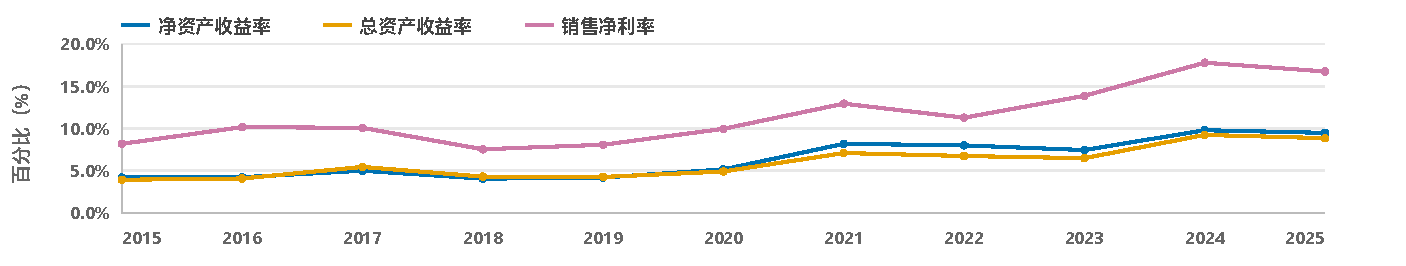
\includegraphics[width=\linewidth]{charts/600219_profitability_print.pdf}\par\vspace{0mm}
\sbox{\cmtable}{\resizebox{130.0mm}{!}{
{\fontsize{6}{7}\selectfont
\setlength{\tabcolsep}{1pt}
\begin{tabular}{|>{\raggedright\arraybackslash}p{21mm}|*{11}{>{\raggedleft\arraybackslash}p{10mm}|}}
\hline
\rowcolor{headbg}\textbf{指标} & \textbf{2015} & \textbf{2016} & \textbf{2017} & \textbf{2018} & \textbf{2019} & \textbf{2020} & \textbf{2021} & \textbf{2022} & \textbf{2023} & \textbf{2024} & \textbf{2025} \\
\hline
资产总计 & 42,150 & 42,685 & 46,041 & 52,299 & 54,759 & 56,012 & 63,178 & 64,726 & 68,815 & 70,264 & 71,917 \\
\hline
股东权益 & 30,489 & 31,675 & 32,744 & 38,228 & 39,309 & 40,385 & 42,867 & 45,102 & 48,344 & 50,317 & 49,587 \\
\hline
货币资金 & 4,584 & 4,083 & 5,571 & 6,305 & 10,346 & 13,227 & 18,273 & 20,875 & 26,388 & 25,662 & 24,553 \\
\hline
流动资产 & 10,818 & 11,071 & 15,173 & 21,759 & 22,724 & 23,125 & 30,697 & 33,994 & 39,926 & 39,683 & 38,385 \\
\hline
非流动资产 & 31,331 & 31,615 & 30,868 & 30,540 & 32,036 & 32,887 & 32,481 & 30,732 & 28,889 & 30,581 & 33,532 \\
\hline
流动负债 & 6,574 & 6,621 & 7,555 & 9,130 & 10,941 & 10,668 & 15,014 & 13,878 & 14,112 & 13,045 & 13,117 \\
\hline
非流动负债 & 3,276 & 2,541 & 3,825 & 2,911 & 2,270 & 1,057 & 640 & 830 & 675 & 994 & 748 \\
\hline
存货 & 3,840 & 3,836 & 4,564 & 5,241 & 5,118 & 4,624 & 6,429 & 6,436 & 6,272 & 6,470 & 8,131 \\
\hline
固定资产 & 19,001 & 23,228 & 25,975 & 25,010 & 24,598 & 23,192 & 27,504 & 26,381 & 24,433 & 23,168 & 26,057 \\
\hline
商誉 & NA & NA & NA & NA & NA & NA & NA & NA & NA & NA & NA \\
\hline
短期贷款 & 1,828 & 1,349 & 2,512 & 3,940 & 4,864 & 5,073 & 8,092 & 7,350 & 7,533 & 5,514 & 5,029 \\
\hline
长期贷款 & 1,501 & 702 & 356 & 100 & 170 & 350 & NA & 190 & 28 & 200 & NA \\
\hline
\end{tabular}}
}}
\makebox[\linewidth][c]{\usebox{\cmtable}}
\vspace{0mm}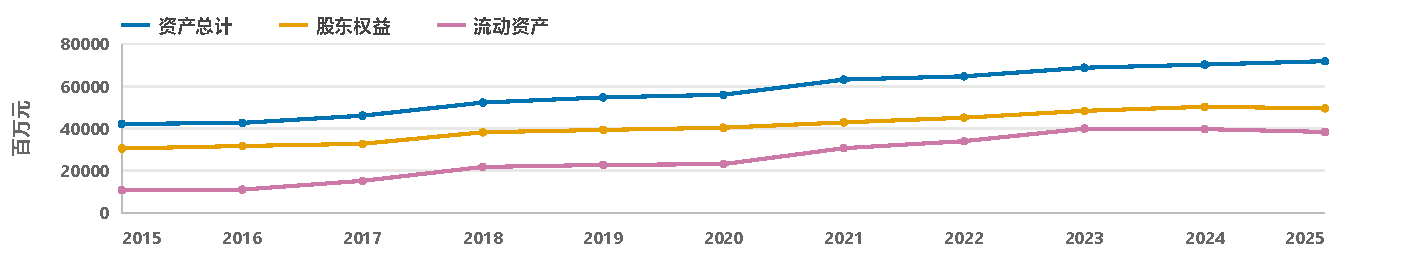
\includegraphics[width=\linewidth]{charts/600219_assets_print.pdf}\par\vspace{0mm}
\sbox{\cmtable}{\resizebox{130.0mm}{!}{
{\fontsize{6}{7}\selectfont
\setlength{\tabcolsep}{1pt}
\begin{tabular}{|>{\raggedright\arraybackslash}p{21mm}|*{11}{>{\raggedleft\arraybackslash}p{10mm}|}}
\hline
\rowcolor{headbg}\textbf{指标} & \textbf{2015} & \textbf{2016} & \textbf{2017} & \textbf{2018} & \textbf{2019} & \textbf{2020} & \textbf{2021} & \textbf{2022} & \textbf{2023} & \textbf{2024} & \textbf{2025} \\
\hline
主营业务收入 & 13,777 & 13,228 & 17,068 & 20,222 & 21,509 & 22,299 & 28,725 & 34,951 & 28,844 & 33,477 & 34,620 \\
\hline
营业利润 & 1,428 & 1,682 & 2,256 & 1,819 & 1,984 & 2,601 & 4,145 & 4,282 & 4,368 & 6,630 & 6,557 \\
\hline
息税前利润 & 1,449 & 1,728 & 2,414 & 2,111 & 2,281 & 2,716 & 4,227 & 4,312 & 4,325 & 6,426 & 6,296 \\
\hline
扣非净利润 & 556 & 529 & 1,599 & 1,372 & 1,448 & 1,947 & 3,337 & 3,826 & 2,715 & 4,908 & 4,610 \\
\hline
归母净利润 & 1,018 & 1,313 & 1,611 & 1,438 & 1,623 & 2,049 & 3,411 & 3,516 & 3,474 & 4,830 & 4,736 \\
\hline
经营净现金流 & 2,631 & 1,892 & 1,810 & 2,184 & 3,792 & 5,883 & 4,416 & 6,669 & 4,230 & 7,617 & 7,429 \\
\hline
现金及等价物净增 & 1,090 & -528 & 1,522 & 407 & 2,723 & 4,001 & 3,274 & 3,572 & 3,049 & 131 & -223 \\
\hline
总股本（百万股） & 2,835 & 9,251 & 9,251 & 11,950 & 11,950 & 11,950 & 11,950 & 11,709 & 11,709 & 11,614 & 11,484 \\
\hline
\end{tabular}}
}}
\makebox[\linewidth][c]{\usebox{\cmtable}}
\vspace{0mm}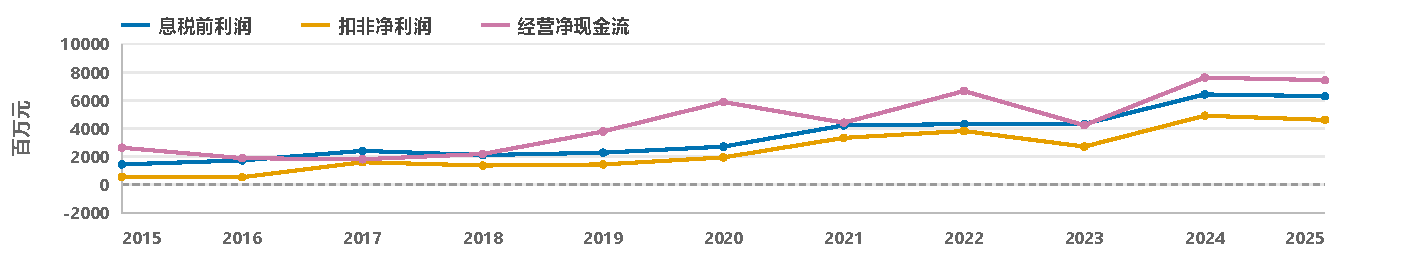
\includegraphics[width=\linewidth]{charts/600219_cashflow_print.pdf}\par\vspace{0mm}
\end{minipage}%
\hspace{0.2mm}%
\begin{minipage}[t]{\dimexpr\textwidth-1.05\cmleftwidth-0.2mm\relax}\vspace{0pt}\setlength{\righttablewidth}{\linewidth}
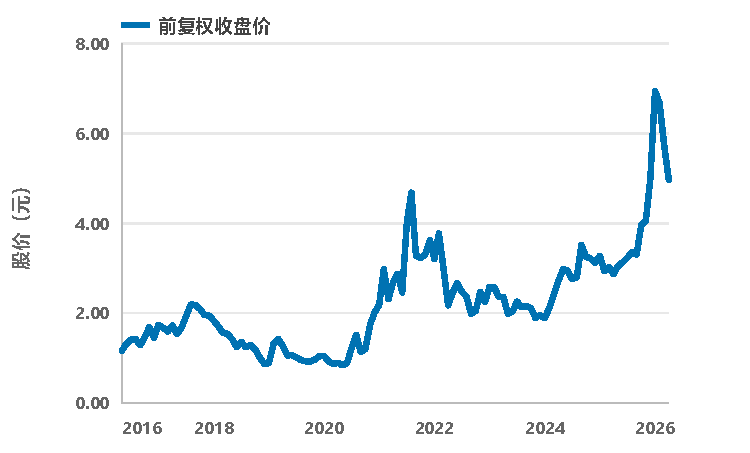
\includegraphics[width=\linewidth]{charts/600219_price_print.pdf}\par
\vspace{-1.4mm}{\centering\fontsize{5.5}{6.5}\selectfont 股价走势（月线，前复权）\\[0.1mm] 2016-05-06 \textasciitilde{} 2026-05-06\par}
\vspace{0.2mm}
\vspace{0.4mm}{\centering\textbf{\fontsize{10}{12}\selectfont 南山铝业}\par}
{\fontsize{6.3}{7.6}\selectfont
\begin{tabularx}{\righttablewidth}{|>{\raggedright\arraybackslash}p{15mm}|>{\raggedright\arraybackslash}X|}
\hline
公司全称 & 山东南山铝业股份有限公司 \\
\hline
所在城市 & 龙口市 \\
\hline
成立日期 & 19930318 \\
\hline
上市日期 & 19991223 \\
\hline
所属行业 & 铝 \\
\hline
主营业务 & 铝及铝合金制品的开发、生产、加工及销售;电力生产。 \\
\hline
\end{tabularx}}
\vspace{0.7mm}\textbf{\fontsize{6.5}{7.5}\selectfont 年均增长率}\par\vspace{0.2mm}
\resizebox{\righttablewidth}{!}{%
{\fontsize{6.3}{7.3}\selectfont
\begin{tabular}{|>{\raggedright\arraybackslash}p{16mm}|*{4}{>{\raggedleft\arraybackslash}p{11mm}|}}
\hline
\rowcolor{headbg}\textbf{时间段} & \textbf{10年} & \textbf{8年} & \textbf{5年} & \textbf{3年} \\
\hline
主营营收 & 9.65\% & 9.24\% & 9.20\% & -0.32\% \\
\hline
净利润 & 16.62\% & 14.43\% & 18.23\% & 10.44\% \\
\hline
总资产 & 5.49\% & 5.73\% & 5.13\% & 3.57\% \\
\hline
股东权益 & 4.98\% & 5.32\% & 4.19\% & 3.21\% \\
\hline
\end{tabular}}
}
\vspace{0.7mm}\textbf{\fontsize{6.5}{7.5}\selectfont 季度营收（百万元，累计值）}\par\vspace{0.2mm}
\resizebox{\righttablewidth}{!}{%
{\fontsize{6}{7}\selectfont
\begin{tabular}{|>{\centering\arraybackslash}p{9mm}|*{4}{>{\raggedleft\arraybackslash}p{12.5mm}|}}
\hline
\rowcolor{headbg}\textbf{年度} & \textbf{一季度} & \textbf{二季度} & \textbf{三季度} & \textbf{四季度} \\
\hline
2026 & 9,067 & NA & NA & NA \\
\hline
2025 & 8,981 & 17,274 & 26,325 & 34,620 \\
\hline
2024 & 7,224 & 15,667 & 24,226 & 33,477 \\
\hline
2023 & 6,834 & 14,501 & 21,690 & 28,844 \\
\hline
2022 & 8,857 & 17,910 & 26,528 & 34,951 \\
\hline
\end{tabular}}
}
\vspace{0.7mm}\textbf{\fontsize{6.5}{7.5}\selectfont 季度净利润（百万元，累计值）}\par\vspace{0.2mm}
\resizebox{\righttablewidth}{!}{%
{\fontsize{6}{7}\selectfont
\begin{tabular}{|>{\centering\arraybackslash}p{9mm}|*{4}{>{\raggedleft\arraybackslash}p{12.5mm}|}}
\hline
\rowcolor{headbg}\textbf{年度} & \textbf{一季度} & \textbf{二季度} & \textbf{三季度} & \textbf{四季度} \\
\hline
2026 & 1,101 & NA & NA & NA \\
\hline
2025 & 1,704 & 2,625 & 3,772 & 4,736 \\
\hline
2024 & 851 & 2,189 & 3,490 & 4,830 \\
\hline
2023 & 519 & 1,313 & 2,142 & 3,474 \\
\hline
2022 & 722 & 1,826 & 2,849 & 3,516 \\
\hline
\end{tabular}}
}
\vspace{0.7mm}\textbf{\fontsize{6.5}{7.5}\selectfont 每股分红（元）}\par\vspace{0.2mm}
\resizebox{\righttablewidth}{!}{%
{\fontsize{6.3}{7.3}\selectfont
\begin{tabular}{|>{\centering\arraybackslash}p{17mm}|*{3}{>{\raggedleft\arraybackslash}p{13mm}|}}
\hline
\rowcolor{headbg}\textbf{年度} & \textbf{现金} & \textbf{送股} & \textbf{转增} \\
\hline
20251231 & 0.14 & NA & NA \\
\hline
20241231 & 0.09 & NA & NA \\
\hline
20231231 & 0.12 & NA & NA \\
\hline
20221231 & 0.04 & NA & NA \\
\hline
\end{tabular}}
}
\end{minipage}
\vspace{1.5mm}\hrule\vspace{1mm}
{\fontsize{5}{6}\selectfont
\noindent\begin{minipage}[t]{0.46\textwidth}报告指标日期为 2026-05-06（报告日最近交易日）；当前股价/市值取该日收盘价与最新披露股本。静态 PE/PB 按 2025 年报计算；动态 PE 按 TTM 归母净利润计算；市净率按 2026-03-31 归母股东权益计算。\end{minipage}\hfill
\begin{minipage}[t]{0.52\textwidth}数据来源：腾讯财经（行情、K 线）；新浪财经（财报三表、公司资料、行业）；东方财富（扣非净利润、分红报告期、北交所 K 线兜底）。本资料所有数据均来源于可靠的公开资料，但无法确保完全准确。如有错讹，概不负责。本资料仅适用于个人投资者训练投资能力，未获授权，禁止一切形式的复制、转载和交易。\end{minipage}
}
\end{document}